%%%%%%%%%%%%%%%%%%%%%%%%%%%%%%%%%%%%%%%%%%%%%%%%%%%%%%%%%%%%%%%%%%%%%%%%%%%%%%
\section{Images of Fabricated Devices}

\begin{figure}[h]
\centering
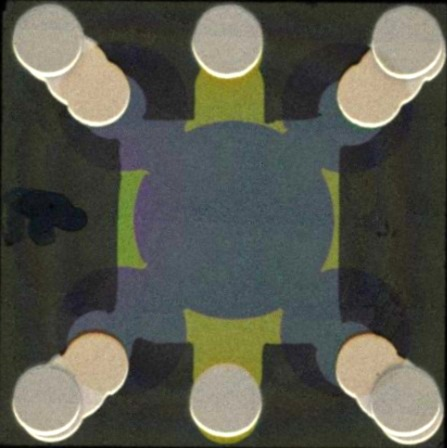
\includegraphics[angle=90,height=50mm]{figures/good-device.jpg}
\hspace{4mm}
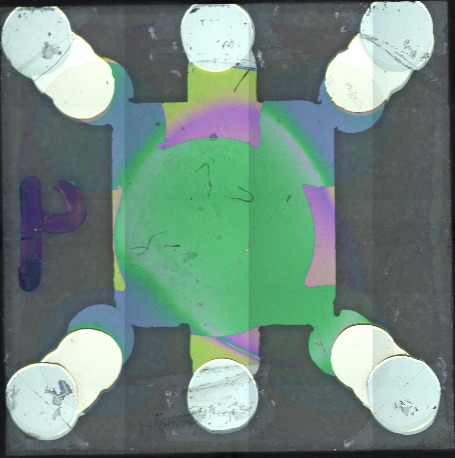
\includegraphics[angle=90, height=50mm]{figures/bad-device.jpg}
\caption[Fabricated devices under the microscope]{Fabricated devices under the microscope. Left: optically well-defined device. Right: device with visible defects. Photos from internal laboratory archive.}
\label{fig:fabricated_devices}
\end{figure}

After fabrication, the devices were inspected under an optical microscope because their electrical behavior depends strongly on the integrity of the active film and the separation of the four contacts~\cite{Sirringhaus2005DevicePhysics,Rolin2017GVDP}. A device was considered suitable for measurement when the semiconductor layer was continuous, the injection contacts were clearly separated, and the contact pads could be reached reliably with the probes.

Figure~\ref{fig:fabricated_devices} shows an optically well-defined device and a defective device. In a well-defined device, the layers are aligned so that the four contacts overlap the semiconductor without shorting neighboring contacts, and the central semiconductor region is continuous. Defective devices can show interrupted metal paths, incomplete semiconductor coverage, mask misalignment, dust particles, or unwanted metal bridges, which may cause open contacts, short circuits, leakage currents, or non-reproducible results.

Optical inspection was followed by electrical checks. The resistance between contact pads was measured to identify open and short circuits, and gate leakage was checked before large gate voltages were applied. Only devices that passed these tests were used for the gVDP measurements described in the following chapters~\cite{Rolin2017GVDP,Lee2024GVDPIGZO}.
